\section{
    Анализ оптимизационного метода решения
    задачи сложного теплообмена с граничными условиями типа коши
}\label{sec:ch3:sec2}

\subsection{Введение}\label{subsec:ch3:sec2:subsec1}
Процедура эндовенозной лазерной абляции (EVLA) безопасна и достаточно
эффективна при лечении варикозного расширения вен [1].
Во время ЭВЛА в поврежденную вену вводится лазерное оптическое волокно.
Затем лазерное излучение передается по волокну, которое в это время вытягивается из вены.
Конец оптического волокна обычно покрыт карбонизированным слоем (наконечник оптического волокна).
Карбонизированный слой разделяет лазерную энергию на нагрев наконечника оптического волокна и излучение.
Тепло от наконечника оптического волокна передается крови за счет кондуктивного теплообмена,
теплопередача значительно увеличивается за счет потока пузырьков,
образующихся на нагретом наконечнике волокна.
Излучение, попадающее в кровь и окружающие ткани, частично поглощается с выделением тепла.
В результате генерируемая тепловая энергия вызывает значительный нагрев вены,
что приводит к ее облитерации (закрытию вены).


Математическое моделирование радиационных и тепловых процессов, возникающих при ЭВЛА,
важно для определения оптимальных параметров излучения, обеспечивающих достаточно
высокую температуру внутри вены для успешной облитерации, с другой стороны,
генерируемое температурное поле должно быть относительно безопасным для тканей, окружающих вену.
Результаты численного моделирования EVLA для длин волн в диапазоне от
810 до $1470 \mathrm{~нм}$ и различных диаметров жил обсуждаются в [2-4].
В [5] отмечается важность математического моделирования для выбора оптимальной
мощности лазерного излучения и скорости отката волокна.
Обычно при выборе оптимальных параметров излучения
используется прямое множественное моделирование [2-5].
Такой подход неэффективен с практической точки зрения.
Более того, вопросы, связанные с существованием и
уникальностью оптимального режима, остаются открытыми.


Наиболее перспективным подходом к выбору оптимальных параметров излучения является
рассмотрение задачи оптимального управления для уравнений
реакционно-диффузионного типа, описывающих процедуру EVLA.
Различные подходы к анализу и оптимизации параметров реакционно-диффузионных моделей,
описывающих различные природные явления, можно найти в [6-9].

Задачи оптимального управления для модели EVLA рассмотрены в [10,11].
В [10] ставится задача оптимального управления для реакционно-диффузионной модели,
описывающей процедуру EVLA, которая заключается в аппроксимации заданного температурного
профиля в определенной точке модельной области.
В [11] изучается аналогичная [10] задача оптимального управления.
Здесь целевой функционал берется таким образом, что его минимизация позволяет достичь
заданного распределения температуры в разных частях модельной области.
Это позволяет обеспечить достаточно высокую температуру внутри вены для ее успешной
облитерации и безопасную температуру в перивенозной ткани.
Доказана однозначная разрешимость начально-краевой задачи,
на основе которой показана разрешимость задачи оптимального управления.
Предложен алгоритм нахождения решения задачи оптимального управления.
Его эффективность проиллюстрирована численным примером.


В настоящей работе рассматривается задача оптимального управления для квазилинейных
уравнений радиационно-кондуктивного теплообмена, моделирующих процесс эндовенозной
лазерной абляции в ограниченной области $\Omega$ с отражающей границей $\Gamma=\partial\Omega$.
Проблема заключается в том, чтобы свести к минимуму функционал

\[ J(\theta)=\int_{0}^{T} \int_{G_{1}}\left(\theta-\theta_{d}\right)^{2} d x d t \rightarrow \inf \]

на решениях начально-краевой задачи:

\[
    \begin{aligned}
        &\sigma \partial \theta / \partial t-\operatorname{div}(k(\theta)
        \nabla \theta)-\beta \varphi=u_{1} \chi \\
        &-\operatorname{div}(\alpha \nabla \varphi)+\beta \varphi=u_{2}
        \chi, \quad x \in \Omega, \quad t \in(0, T), \\
        &\theta=\left.0\right|_{\Gamma}, \quad \alpha \partial_{n}
        \varphi+\left.2^{-1} \varphi\right|_{\Gamma}=0,\left.\quad \theta\right|_{t=0}=\theta_{0}
    \end{aligned}
\]

При этом учитываются ограничения:

\[
    u_{1,2} \geq 0, \quad u_{1}+u_{2} \leq P,\left.\quad \theta\right|_{G_{2}} \leq \theta_{*}
\]

Здесь $G_{1}$ и $G_{2}$ подмножества $\Omega, \theta$
представляет собой разницу между реальной температурой
(в единицах Цельсия) и постоянной граничной температурой,
$\varphi$ является ли интенсивность излучения усредненной по всем направлениям, $\alpha$
является коэффициентом диффузии фотонов, $\beta$ является коэффициентом поглощения,
$k(\theta)$ является коэффициентом теплопроводности, $\sigma(x, t)$
является произведением удельной теплоемкости и объемной плотности, $u_{1}$
описывает мощность источника, затрачиваемую на нагрев наконечника волокна, $u_{2}$
это мощность источника, расходуемая на излучение,
$P$ является максимальной мощностью лазерного источника, $\chi$
является характерной функцией той части среды, в которой волокно
наконечник расположен деленным на объем волоконного наконечника.
Обратите внимание, что значения параметров $u_{1}$ and $u_{2}$
определяются методом карбонизации кончика волокна.
Обзор некоторых способов карбонизации приведен в $[10]$.

Таким образом, при моделировании процедуры EVLA мы будем использовать диффузионную модель,
которая учитывает кондуктивный теплообмен, а также перенос излучения и поглощение с выделением тепла.
Поток пузырьков, образующихся на нагретом наконечнике оптического волокна, вносит значительный
вклад в температурное поле. В [2-4], основываясь на оценке экспериментальных данных,
теплопередача потоком пузырьков моделируется с использованием кусочно-постоянного
коэффициента теплопроводности, который зависит от температуры следующим образом:
когда температура в некоторой точке достигает $95 ^ {\circ} \mathrm{C}$,
коэффициент теплопроводность увеличивается в 200 раз.

Следуя задаче оптимального управления, требуется обеспечить заданное распределение
температурного поля $\theta_{d}$ в поддомене $G_{1}$,
при этом температура в поддомене $G_{2}$ не может превышать
(если это возможно) критическое значение $\theta_{*}=$ Const $>0$.


\subsection{Формализация задачи оптимального управления}
\label{subsec:ch3:sec2:subsec2}

Будем далее предполагать, что $\Omega$ является липшицевой ограниченной областью,
$\Gamma=\partial \Omega, Q=\Omega \times(0, T)$, $\Sigma=\Gamma \times(0, T)$.
Обозначим через $L^{p}, 1 \leq p \leq \infty$, пространство Лебега,
через $H^{1}$ пространство Соболева $W_{2}^{1}$,
через $H_{ 0}^{1}$ подпространство функций из $H^{1}$ с нулевыми граничными значениями,
а через $L^{p}(0, T ; X)$ пространство Лебега функций из $L^{ p}$,
определенный на $(0, T)$, со значениями в банаховом пространстве $X$.

Пусть $H=L^{2}(\Omega), V=H_{0}^{1}(\Omega)$, а пространство $V^{\prime}$ двойственно к $V$.
Затем мы отождествляем $H$ с его двойственным пространством $H^{\prime}$ таким,
что $V \subset H^{1}(\Omega) \subset H=H^{\prime} \subset$
$\left( H^{1}(\Omega)\right)^{\prime} \subset V^{\prime}$,
и обозначим через $\|\cdot\|$ норму в $H$,
а через $(h , v)$ значение функционала $h \in V^{\prime}$
на элементе $v \in V$, совпадающее со скалярным произведением в $H$, если $h \in H$.
Скалярный продукт в $V$ определяется как $(u, v)_{V}=(\nabla u, \nabla v)$.


Будем предполагать, что выполнены следующие условия:

(c1) $\sigma_{0} \leq \sigma \leq \sigma_{1}, \quad|\partial \sigma / \partial t| \leq \sigma_{2}$

(c2) $k_{0} \leq k(s) \leq k_{1}, \quad\left|k^{\prime}(s)\right| \leq k_{2}, \quad s \in \mathbb{R}$,

(c3) $\theta_{0} \in H$

(c4) $\alpha_{0} \leq \alpha(x) \leq \alpha_{1}, \beta_{0} \leq \beta(x) \leq \beta_{1}, \quad x \in \Omega$,

где $\sigma_{i}, k_{i}, \alpha_{i}$, и $\beta_{i}$ положительные константы.

Определим нелинейный оператор $A: V \rightarrow V^{\prime}$ и линейный оператор
$B: H^{1}(\Omega) \rightarrow\left(H^{1}(\Omega)\right)^{\prime}$
используя следующие равенства, справедливые для любого
$\theta, v \in V, \varphi, w \in$ $H^{1}(\Omega)$

\[
    \begin{aligned}
        &(A(\theta), v)=(k(\theta) \nabla \theta, \nabla v)=(\nabla h(\theta), \nabla v) \\
        &(B \varphi, w)=(\alpha \nabla \varphi, \nabla w)+(\beta \varphi, w)+2^{-1}
        \int_{\Gamma} \varphi w d \Gamma
    \end{aligned}
\]

где
\[
    h(s)=\int_{0}^{s} k(r) d r.
\]

\textbf{Definition 1.} Пусть $u_{1,2} \in L^{2}(0, T)$.
Пара функций $\theta \in L^{2}(0, T ; V), \varphi \in L^{2}\left(0, T ; H^{1}(\Omega)\right)$
тогда $a$ ялвяется слабым решением задачи (1), (2)
если $\sigma \theta^{\prime} \in$ $L^{2}\left(0, T ; V^{\prime}\right)$ и

$\sigma \theta^{\prime}+A(\theta)-\beta \varphi=u_{1} \chi, \quad \theta(0)=\theta_{0},
\quad B \varphi=u_{2} \chi$ where $\theta^{\prime}=d \theta / d t$.
Из леммы Лакса-Мильграма следует, что для любой функции $g \in H$ существует единственное
решение уравнения $B \varphi=g$.
Более того, обратный оператор $B^{-1}: H \rightarrow H^{1}(\Omega)$ непрерывен.
Поэтому можно исключить интенсивность излучения $\varphi=u_{2} B^{-1} \chi$ и
сформулировать задачу оптимального управления следующим образом.


\subsection{Problem (P)}
\label{subsec:ch3:sec2:subsec3}
\[
    J(\theta)=\int_{0}^{T}
    \int_{G_{1}}\left(\theta-\theta_{d}\right)^{2} d x d t \rightarrow \inf
\]

\[
    \begin{aligned}
        & \sigma \theta^{\prime}+A(\theta)=u,
        \quad \theta(0)=\theta_{0},\left.\quad
        \theta\right|_{G_{2}} \leq \theta_{*},
        \quad u \in U_{a d},
    \end{aligned}
\]

где

\[
    \begin{array}{r}
        U_{a d}=\left\{u=u_{1} \chi+u_{2} \beta B^{-1}
        \chi: u_{1,2} \in L^{2}(0, T),\right. \\
        \left.u_{1,2} \geq 0, u_{1}+u_{2} \leq P\right\}
    \end{array}
\]


\subsection{Предварительные результаты}
\label{subsec:ch3:sec2:subsec4}
Давайте рассмотрим проблему
\[
    \sigma \theta^{\prime}+A(\theta)=f, \quad \theta(0)=\theta_{0}.
\]
Справедлива следующая лемма [11].

\textit{Lemma 1.}
Пусть выполняются условия (c1)-(c3) и $f \in$ $L^{2}\left(0, T ; V^{\prime}\right)$.
Тогда существует решение задачи (3) такое, что $\theta \in L^{\infty}(0, T ; H)$
и справедливы следующие оценки:
\[
    \begin{gathered}
        \|\theta(t)\|^{2} \leq \frac{K}{\sigma_{0}} \exp \frac{\sigma_{2} t}{\sigma_{0}}
        \quad \text { a.e. on }(0, T) \\
        \int_{0}^{T}\|\theta(t)\|_{V}^{2} d t \leq
        \frac{K}{k_{0}}\left(1+\frac{\sigma_{2} T}{\sigma_{0}} \exp
        \frac{\sigma_{2} T}{\sigma_{0}}\right)
    \end{gathered}
\]

где $K=\sigma_{1}\left\|\theta_{0}\right\|^{2}
+ k_{0}^{-1}\|f\|_{L^{2}\left(0, T; V^{\prime}\right)}^{2}$.

Следующий результат важен для установления непустоты множества допустимых пар управляющих состояний.
\textit{Lemma 2.}Пусть выполняются условия (c1)-(c3) и
$f=0$, $\theta_{0} \leq \theta_{*}$ a.e. в $\Omega$, и $\theta$ решение задачи (3).
Тогда $\theta \leq \theta_{*}$ a.e. в $\Omega \times(0, T)$.

\textbf{Proof.}
Скалярно умножим в $H$ первое уравнение $(3)$ на
$v=\max \{\theta-$ $\left.\theta_{*}, 0\right\} \in L^{2}(0, T ; V)$ получаем

\[ \left(\sigma v^{\prime}, v\right)+(k(\theta) \nabla v, \nabla v)=0. \]

Отбрасывая неотрицательный второй член, приходим к оценке
\[ \frac{d}{d t}(\sigma v, v) \leq\left(\sigma_{t} v, v\right) \leq \sigma_{2}\|v\|^{2} . \]
Учитывая, что $\left.v\right|_{t=0}=0$,проинтегрировать последнее неравенство по времени.
Тогда
\[ \sigma_{0}\|v(t)\|^{2} \leq(\sigma v(t), v(t)) \leq \sigma_{2} \int_{0}^{t}\|v(\tau)\|^{2} d \tau \]

На основании леммы Гронуолла заключаем,
что $v=0$ и, следовательно, $\theta \leq \theta_{*}$ почти всюду в $\Omega\times(0,T)$.

\subsection{Разрешимость задачи оптимального управления}
\label{subsec:ch3:sec2:subsec5}

\textbf{Theorem 1.}
Пусть выполняются условия (c1)-(c3), и $\theta_{0} \leq \theta_{*}$ a.e. в $\Omega$.
Тогда существует решение задачи $(\mathrm{P})$.

\textbf{Proof.}
Согласно леммам 1 и 2 множество допустимых пар непусто.
Рассмотрим минимизирующую последовательность допустимых
пар $\left\{\theta_{m}, u_{m}\right\} \in$ $L^{2}(0, T ; V) \times U_{a d}$
такой, что $J\left(\theta_{m}\right) \rightarrow j=\inf J$, где
\[
    \sigma \theta_{m}^{\prime}+A\left(\theta_{m}\right)=u_{m},
    \quad \theta_{m}(0)=\theta_{0},\left.\quad \theta_{m}\right|_{G_{2}} \leq \theta_{*} .
\]

Ограниченность в $L^{2}(0, T ; H)$ множества допустимых управлений $U_{a d}$ влечет по лемме 1 оценки:

\[
    \begin{gathered}
        \left\|\theta_{m}\right\|_{L^{\infty}(0, T ; H)} \leq C,
        \quad\left\|\theta_{m}\right\|_{L^{2}(0, T ; V)} \leq C, \\
        \left\|h\left(\theta_{m}\right)\right\|_{L^{2}(0, T ; V)} \leq C.
    \end{gathered}
\]

Здесь и далее при доказательстве теоремы через $C$ обозначаются константы, не зависящие от $m$.
Оценки (5), используя при необходимости подпоследовательности,
приводят к существованию функций
$u \in U_{a d}, \quad \theta \in L^{2}(0, T ; V)$, $\chi  \in L^{2}(0, T; V)$
такое, что

\[
    \begin{aligned}
        & u_{m} \rightarrow u \text { weakly in } L^{2}(0, T ; H), \\
        & \theta_{m} \rightarrow \theta \text { weakly in } L^{2}(0, T ; V) \text {, } \\
        & \text { *-weakly in } L^{\infty}(0, T ; H) \text {, } \\
        & h\left(\theta_{m}\right) \rightarrow \chi \text { weakly in } L^{2}(0, T ; V) \text {. }
    \end{aligned}
\]

Результаты сходимости (6) достаточны для предельного перехода
при $m \rightarrow \infty$ в системе (4) и доказательства того,
что предельная функция $\theta \in L^{2}(0, T ; V) $ такова,
что $\sigma \theta^{\prime} \in L^{2}\left(0, T ; V^{\prime}\right)$ удовлетворяет равенству

\[ \left(\sigma \theta^{\prime}, v\right)+(\nabla \chi, \nabla v)=(u, v) \quad \forall v \in V \]

и начальное условие верно.

Следующая оценка гарантирует компактность последовательности $\theta_{m}$ in $L^{2}(Q)$:
\[ \int_{0}^{T-\delta}\left\|\theta_{m}(s+\delta)-\theta_{m}(s)\right\|^{2} d s \leq C \delta \]

Из неравенства (7), используя при необходимости подпоследовательности, получаем, что
$\theta_{m} \rightarrow \theta$ in $L^{2}(Q)$.
Следовательно, в силу неравенства

\[ \left|h\left(\theta_{m}\right)-h(\theta)\right| \leq k_{1}\left|\theta_{m}-\theta\right|, \]
следует, что $h\left(\theta_{m}\right) \rightarrow h(\theta)$ in $L^{2}(Q)$
и, следовательно $\chi=h(\theta)$.
Кроме того, предельная функция $\theta$ удовлетворяет неравенству
$\left.\theta\right|_{G_{2}} \leq \theta_{*}$.
Следовательно, допустима предельная пара $\{\theta, u\} \in L^{2}(0, T ; V) \times U_{a d}$.
Поскольку функционал $J$ слабо полунепрерывен снизу,

\[ j \leq J(\theta) \leq \liminf J\left(\theta_{m}\right)=j, \]

тогда пара $\{\theta, u\}$ является решением задачи $(\mathrm{P})$.


\subsection{Задача штрафов}

Чтобы численно решить задачу оптимального управления с фазовыми ограничениями
$\left.\theta\right|_{G_{2}} \leq \theta_{*}$, рассмотрим следующую задачу штрафов.

$\operatorname{Problem}\left(\mathbf{P}_{\varepsilon}\right): J_{\varepsilon}(\theta) \rightarrow \inf$,
где
\[
    \begin{aligned}
        & J_{\varepsilon}(\theta)=\int_{0}^{T} \int_{G_{1}}\left(\theta-\theta_{d}\right)^{2} d x d t \\
        & +\frac{1}{\varepsilon} \int_{0}^{T} \int_{G_{2}} F(\theta) d x d t, \\
        & \sigma \theta^{\prime}+A(\theta)=u, \quad \theta(0)=\theta_{0}, \quad u \in U_{a d} .
    \end{aligned}
\]

Здесь,
\[
    F(\theta)= \begin{cases}
                   0, & \text { if } \theta \leq \theta_{*} \\
                   \left(\theta-\theta_{*}\right)^{2}, & \text { if } \theta>\theta_{*}
    \end{cases}
\]
Оценки, представленные в лемме 1, также позволяют доказать разрешимость
задачи со штрафом аналогично доказательству теоремы 1.

\textbf{Theorem 2.}
Пусть выполняются условия (c1)-(c3).
Тогда существует решение задачи $\left(\mathrm{P}_{\varepsilon}\right)$.

Рассмотрим аппроксимативные свойства решений задачи со штрафом.
Пусть $\left\{\theta_{\varepsilon}, u_{\varepsilon}\right\}$ — решения задачи
$\left(\mathrm{P}_{\varepsilon}\right)$ и $\{\ theta, u\}$
— решение задачи $(\mathrm{P})$.
Затем,

\[
    \sigma \theta_{\varepsilon}^{\prime}+A\left(\theta_{\varepsilon}\right)=u_{\varepsilon},
    \quad \theta_{\varepsilon}(0)=\theta_{0} .
\]

Since $\left.\theta\right|_{G_{2}} \leq \theta_{*}$, the following inequality is true:

\[
    \begin{array}{r}
        \int_{0}^{T} \int_{G_{1}}\left(\theta_{\varepsilon}-\theta_{d}\right)^{2} d x d t+\frac{1}{\varepsilon}
        \int_{0}^{T} \int_{G_{2}} F\left(\theta_{\varepsilon}\right) d x d t \\
        \leq \int_{0}^{T} \int_{G_{1}}\left(\theta-\theta_{d}\right)^{2} d x d t=J(\theta)
    \end{array}
\]
Следовательно,
\[
    \begin{aligned}
        &\int_{0}^{T} \int_{G_{1}}\left(\theta_{\varepsilon}-\theta_{d}\right)^{2} d x d t \leq J(\theta) \\
        &\int_{0}^{T} \int_{G_{2}} F\left(\theta_{\varepsilon}\right) d x d t \leq \varepsilon J(\theta)
    \end{aligned}
\]
Из полученных оценок, используя при необходимости подпоследовательности,
соответствующие $\varepsilon_{k} \rightarrow+0$,
аналогично доказательству теоремы 1, устанавливаем существование
функций $\widehat{u} \in U_{a d}, \widehat{\theta} \in L^{2}(0, T ; V)$, такой, что

\[
    \begin{aligned}
        u_{\varepsilon} & \rightarrow \widehat{u} \text { weakly in } L^{2}(0, T ; H) \\
        \theta_{\varepsilon} \rightarrow \widehat{\theta} \text { weakly in } L^{2}(0, T ; V) \\
        & \text { strongly in } L^{2}(0, T ; H) .
    \end{aligned}
\]
Заметим, что

\[
    \begin{aligned}
        &\int_{0}^{T} \int_{G_{2}} F\left(\theta_{\varepsilon}\right) d x d t
        \rightarrow \int_{0}^{T} \int_{G_{2}} F(\widehat{\theta}) d x d t \\
        &\int_{0}^{T} \int_{G_{2}} F\left(\theta_{\varepsilon}\right) d x d t
        \rightarrow 0, \text { as } \varepsilon \rightarrow+0
    \end{aligned}
\]

что гарантирует, что $F(\widehat{\theta})=0$ and $\left.\widehat{\theta}\right|_{G_{2}} \leq \theta_{*}$.

Результаты сходимости достаточны для предельного перехода по $\varepsilon \rightarrow+0$ в системе (8)
и доказательства того, что предельная пара
$\{\widehat{\theta}, \widehat{u}\} \in L ^{2}(0, T ; V) \times U_{a d}$
допустимо для задачи $(\mathrm{P})$.
Поскольку функционал $J$ слабо полунепрерывен снизу,

\[
    j \leq J(\widehat{\theta}) \leq \liminf J\left(\theta_{\varepsilon}\right) \leq J(\theta)=j=\inf J,
\]

тогда пара $\{\widehat{\theta}, \widehat{u}\}$ есть решение задачи $(\mathrm{P})$.

\textbf{Theorem 3.}
Пусть выполнены условия (c1)-(c3), и $\theta_{0} \leq \theta_{*}$ a.e. in $\Omega$.
Если $\left\{\theta_{\varepsilon}, u_{\varepsilon}\right\}$ есть решения проблемы
$\left(\mathrm{P}_{\varepsilon}\right)$ for $\varepsilon>0$, тогда существует
такая последовательность$\varepsilon \rightarrow+0$ что


\[
    \begin{aligned}
        &u_{\varepsilon} \rightarrow \widehat{u} \text { weakly in } L^{2}(0, T ; H) \\
        &\theta_{\varepsilon} \rightarrow \widehat{\theta} \text { strongly in } L^{2}(0, T ; H),
    \end{aligned}
\]


где $\{\widehat{\theta}, \widehat{u}\}$ есть решение проблемы $(\mathrm{P})$.


\subsection{Реализация численного алгоритма}

Рассмотрим итерационный алгоритм решения задачи оптимального управления
$\left(\mathrm{P}_{\varepsilon}\right)$ для случая, когда параметры управления
$u_{1}$ и $u_{2}$ не зависят от времени.
На каждой итерации алгоритма
решается линейно-квадратичная задача оптимального управления, в которой требуется найти минимум функционала:

\[
    \begin{aligned}
        &\widehat{J}_{\varepsilon}(\theta)=\int_{0}^{T} \int_{G_{1}}\left(\theta-\theta_{d}\right)^{2} d x d t \\
        &+\frac{1}{\varepsilon} \int_{0}^{T}
        \int_{G_{*}}\left(\theta-\theta_{*}\right)^{2} d x d t \rightarrow \inf , \quad u \in U_{a d}
    \end{aligned}
\]

с соответствующими ограничениями
\[
    \begin{aligned}
        &\sigma \partial \theta / \partial t-\operatorname{div}(k(\widehat{\theta})
        \nabla \theta)=u, \quad x \in \Omega, \quad 0<t<T, \\
        &\left.\theta\right|_{\Gamma}=0, \quad \theta(x, 0)=\theta_{0} .
    \end{aligned}
\]

Здесь,
\[
    \begin{gathered}
        U_{a d}=\left\{u=u_{1} \chi+u_{2} \beta B^{-1} \chi: u_{1,2} \in \mathbb{R},\right. \\
        \left.u_{1,2} \geq 0, u_{1}+u_{2} \leq P\right\}, \\
        G_{*}=\left\{x \in G_{2}: \hat{\theta}(x, t)>\theta_{*}\right\} .
    \end{gathered}
\]

Функция $\widehat{\theta}$ описывает поле температуры, найденное на предыдущей итерации.

В качестве зависимости коэффициента теплопроводности от температуры используется
гладкая аппроксимация кусочно-постоянной функции, рассмотренной в $[2-4]$.

Как легко видеть, задача (9), (10) сводится к нахождению минимума
квадратичной функции параметров $u_{1}$ и $u_{2}$:


\[
    \widehat{J}_{\varepsilon}\left(u_{1} \Theta_{1}+u_{2} \Theta_{2}+\Theta_{3}\right) \rightarrow \inf
\]

на треугольнике  $\left\{u_{1}, u_{2} \in \mathbb{R}: u_{1,2} \geq 0, u_{1}+u_{2} \leq P\right\}$.
Функции $\Theta_{1}, \Theta_{2}$ и $\Theta_{3}$ вычисляются заранее как решения следующих линейных
начально-краевых задач для $x \in \Omega, t \in(0 , Т)$ :


\[
    \begin{aligned}
        &\sigma \partial \Theta_{1} / \partial t-\operatorname{div}\left(k(\widehat{\theta})
        \nabla \Theta_{1}\right)=\chi, \\
        &\left.\Theta_{1}\right|_{\Gamma}=0, \quad \Theta_{1}(x, 0)=0 \\
        &\sigma \partial \Theta_{2} / \partial t-\operatorname{div}\left(k(\widehat{\theta})
        \nabla \Theta_{2}\right)=\beta B^{-1} \chi, \\
        &\left.\Theta_{2}\right|_{\Gamma}=0, \quad \Theta_{2}(x, 0)=0 \\
        &\sigma \partial \Theta_{3} / \partial t-\operatorname{div}\left(k(\widehat{\theta})
        \nabla \Theta_{3}\right)=0 \\
        &\left.\Theta_{3}\right|_{\Gamma}=0, \quad \Theta_{3}(x, 0)=\theta_{0} .
    \end{aligned}
\]

При проведении численных экспериментов использовалась модельная область в
цилиндрической системе координат с угловой симметрией, как показано на рис. 1.
Толщина карбонизированного слоя равна
$0,2 \mathrm{~мм}$, скорость вытягивания волокна
$2 \mathrm{~мм}/\mathrm{s}$. Рассматривалось излучение с длиной волны
$1064 \mathrm{~нм}$.
Оптические и теплофизические параметры среды взяты из $[2-4]$.


Для демонстрации сходимости итерационного алгоритма в качестве
решения прямой начально-краевой задачи для $\left(u_{1}, u_{2}\right)=( 3,7)$
(здесь и далее единицы в ваттах).
Области $G_{1}$ и $G_{2}$
берутся как достаточно малые окрестности точек $(1.5,10),(3.5,10)$.
Для реализации итерационного алгоритма мы взяли $\varepsilon=0.3$ и $\theta_{*}$,
соответствующие $47^{\circ} \mathrm{C}$.


%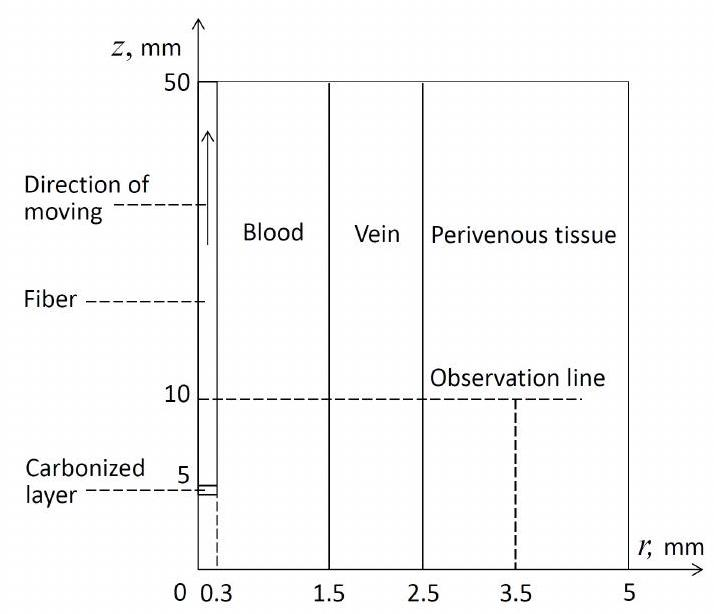
\includegraphics[max width=\textwidth]{2022_10_23_0545711a836d5ec06b12g-5}

Рисунок 1: Область.

%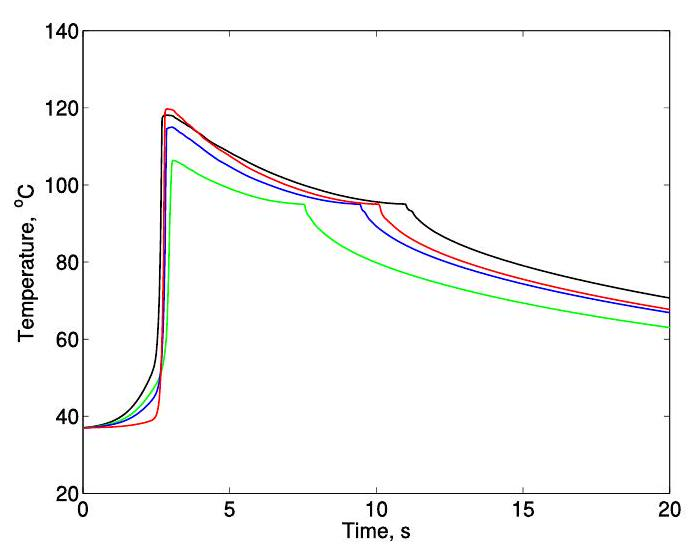
\includegraphics[max width=\textwidth]{2022_10_23_0545711a836d5ec06b12g-5(1)}

Рисунок 2: Температурные профили: желаемая температура (черный),
1-е (зеленое), 2-е (синее) и 3-е (красное) приближения.

Аппроксимации решения в точке $(1.5,10)$ показаны на рис. 2.
Аппроксимации после 1-го, 2-го и 3-го шагов итерационного алгоритма отмечены зеленым
цветом
$\left(\left(u_{1 }, u_{2}\right)=\right.$ $(2.5,4.8))$,
синим  $\left(\left(u_{1}, u_{2}\right)=(3.4,3.5)\right)$
и красным $\left(\left(u_{1}, u_{2}\right)=(4.2,0.9)\right)$ соответственно.
Черная линия показывает желаемую температуру, соответствующую
$\left(u_{1}, u_{2}\right)=(3,7)$.
Максимальное значение температуры в точке $(3.5,10)$ равно $48,8^{\circ}\mathrm{C}$.
Отметим, что при $\left(u_{1}, u_{2}\right)=(3,7)$ максимальное значение
температуры в точке $(3.5,10)$ равно $50,2^{ \circ} \mathrm{C}$.

Эксперимент демонстрирует возможность снижения температуры в
околовенозной ткани при сохранении температурного режима внутри вены.
